\documentclass[10pt]{article}
\usepackage[margin=2.3cm]{geometry}
\usepackage{amsmath,amssymb,booktabs,graphicx,float,hyperref}
\usepackage[font=small]{caption}
\setlength{\parindent}{0pt}
\setlength{\parskip}{4pt}
\newcommand{\E}{\mathbb{E}}
\newcommand{\Var}{\operatorname{Var}}
\newcommand{\Cov}{\operatorname{Cov}}
\newcommand{\Corr}{\operatorname{Corr}}
\newcommand{\Yh}{\widehat Y}
\newcommand{\Vh}{\widehat V}
\newcommand{\Sh}{\widehat S}
\newcommand{\R}{../results}
\newcommand{\VRFPLa}{1.00}
\newcommand{\GainPLa}{1.00}
\newcommand{\VRFPLb}{1.00}
\newcommand{\GainPLb}{1.00}
\newcommand{\VRFPLc}{1.00}
\newcommand{\GainPLc}{1.00}
\newcommand{\VRFCVa}{2.59}
\newcommand{\GainCVa}{1.90}
\newcommand{\RhoXCCVa}{0.79}
\newcommand{\CoefCVa}{1.14}
\newcommand{\CtrlZCVa}{-0.32}
\newcommand{\VRFCVb}{3.16}
\newcommand{\GainCVb}{2.32}
\newcommand{\RhoXCCVb}{0.83}
\newcommand{\CoefCVb}{0.98}
\newcommand{\CtrlZCVb}{0.00}
\newcommand{\VRFCVc}{3.59}
\newcommand{\GainCVc}{2.63}
\newcommand{\RhoXCCVc}{0.85}
\newcommand{\CoefCVc}{0.93}
\newcommand{\CtrlZCVc}{0.07}
\newcommand{\VRFAVa}{1.10}
\newcommand{\GainAVa}{1.49}
\newcommand{\RhoPairAVa}{-0.12}
\newcommand{\VRFAVb}{1.37}
\newcommand{\GainAVb}{1.86}
\newcommand{\RhoPairAVb}{-0.28}
\newcommand{\VRFAVc}{1.86}
\newcommand{\GainAVc}{2.52}
\newcommand{\RhoPairAVc}{-0.47}
\newcommand{\VRFBOTHa}{2.56}
\newcommand{\GainBOTHa}{2.41}
\newcommand{\RhoPairBOTHa}{-0.11}
\newcommand{\RhoACABOTHa}{0.76}
\newcommand{\CoefBOTHa}{1.16}
\newcommand{\CtrlZBOTHa}{1.11}
\newcommand{\VRFBOTHb}{2.99}
\newcommand{\GainBOTHb}{2.82}
\newcommand{\RhoPairBOTHb}{-0.28}
\newcommand{\RhoACABOTHb}{0.74}
\newcommand{\CoefBOTHb}{1.11}
\newcommand{\CtrlZBOTHb}{0.99}
\newcommand{\VRFBOTHc}{2.75}
\newcommand{\GainBOTHc}{2.59}
\newcommand{\RhoPairBOTHc}{-0.47}
\newcommand{\RhoACABOTHc}{0.58}
\newcommand{\CoefBOTHc}{1.48}
\newcommand{\CtrlZBOTHc}{1.16}
\newcommand{\TimePL}{1.23}
\newcommand{\TimeCV}{1.68}
\newcommand{\TimeAV}{0.91}
\newcommand{\TimeBOTH}{1.30}
\newcommand{\GainSpreadc}{4}
\newcommand{\SEVRFPL}{1.0}
\newcommand{\SEGainPL}{1.0}
\newcommand{\SEVRFCV}{20.4}
\newcommand{\SEGainCV}{14.6}
\newcommand{\SERhoXCCV}{0.975}
\newcommand{\SEVRFAV}{1.9}
\newcommand{\SEGainAV}{2.7}
\newcommand{\SERhoPairAV}{-0.46}
\newcommand{\SEVRFBOTH}{21.1}
\newcommand{\SEGainBOTH}{19.0}
\newcommand{\SERhoPairBOTH}{-0.46}
\newcommand{\SERhoACABOTH}{0.955}
\newcommand{\SHVRFPL}{1.0}
\newcommand{\SHGainPL}{1.0}
\newcommand{\SHVRFCV}{7.1}
\newcommand{\SHGainCV}{5.4}
\newcommand{\SHRhoXCCV}{0.925}
\newcommand{\SHVRFAV}{1.5}
\newcommand{\SHGainAV}{2.3}
\newcommand{\SHRhoPairAV}{-0.33}
\newcommand{\SHVRFBOTH}{8.6}
\newcommand{\SHGainBOTH}{9.0}
\newcommand{\SHRhoPairBOTH}{-0.34}
\newcommand{\SHRhoACABOTH}{0.906}
\newcommand{\TimeCOND}{0.80}
\newcommand{\VRFCOND}{1.76}
\newcommand{\GainCOND}{2.70}


\title{MTH 9821 --- Variance reduction in a rough volatility model}
\author{}
\date{}

\begin{document}
\maketitle
\vspace{-1.2cm}
\begin{center}
Team 9: Jaskaran Kalra, William McDonnell
\end{center}

Equation numbers $(1)$--$(21)$ refer to the assignment. Code: \texttt{src/}; every table and
figure is produced by \texttt{python run\_all.py} (see README).

%=====================================================================
\section*{Problem 1. Build and validate the simulator}

\subsection*{(a)}
\textbf{Moments of $Y_t$.} The integrand $s\mapsto\sqrt{2H}(t-s)^{H-1/2}$ is deterministic and
square integrable on $[0,t]$ because $2H-1>-1$. Hence $Y_t$ is a Wiener integral: Gaussian with
$\E[Y_t]=0$, and by the It\^o isometry
\[
\Var(Y_t)=2H\int_0^t (t-s)^{2H-1}\,ds = 2H\cdot\frac{t^{2H}}{2H}=t^{2H}.
\]
For $Z\sim N(0,v)$, $\E[e^{\eta Z}]=e^{\eta^2 v/2}$, so
$\E[V_t]=\xi e^{-\eta^2t^{2H}/2}\,\E[e^{\eta Y_t}]=\xi$. This is (3).

\textbf{$a_H\in(0,1)$.} $a_H=\sqrt{2H}/(H+\tfrac12)>0$ for $H>0$, and
$a_H<1\iff 2H<(H+\tfrac12)^2\iff 0<(H-\tfrac12)^2$, which holds for $H\neq\tfrac12$, in
particular on $0<H<\tfrac12$. So $\sqrt{1-a_H^2}$ is real.

\textbf{Covariance with $\Delta W_j$.} With $\Delta W_j=\sqrt\Delta G_j$ and $U_j$ independent of $G_j$,
\[
\Cov\!\Big(\Delta^H\big(a_HG_j+\sqrt{1-a_H^2}\,U_j\big),\,\Delta W_j\Big)=\Delta^H a_H\sqrt\Delta
=\frac{\sqrt{2H}}{H+\tfrac12}\,\Delta^{H+1/2}.
\]
The exact most-recent-interval integral is $I_j=\sqrt{2H}\int_{t_{j-1}}^{t_j}(t_j-s)^{H-1/2}dW_s$.
By the It\^o isometry for the covariance of two Wiener integrals ($\Delta W_j=\int_{t_{j-1}}^{t_j}1\,dW_s$),
\[
\Cov(I_j,\Delta W_j)=\sqrt{2H}\int_{t_{j-1}}^{t_j}(t_j-s)^{H-1/2}ds=\frac{\sqrt{2H}}{H+\tfrac12}\Delta^{H+1/2},
\]
which matches. (Also $\Var(I_j)=\Delta^{2H}$, equal to the variance $\Delta^{2H}(a_H^2+1-a_H^2)$ of
the first term of (9); both pairs are jointly Gaussian, so their joint laws agree.)

\subsection*{(b)}
\textbf{Implementation} (\texttt{src/model.py}). $w_k$ and $q_j$ are precomputed. The sum in (9) is
$\sum_{i=1}^{j-1}w_{j-i+1}\Delta W_i$, computed for all $j$ at once as a product of the
$(\text{paths}\times n)$ matrix of $\Delta W$ with a fixed upper-triangular $n\times n$ matrix
$M_{ij}=w_{j-i+1}\mathbf 1\{i<j\}$ (checked against a direct double loop to $10^{-15}$). Then (11)
gives $\Vh_j$, and (12) uses $\Vh_j$, $j=0,\dots,n-1$, with $\Delta W_{j+1},\Delta B_{j+1}$.

\textbf{Derivation of (10).} $\Yh_j$ is a linear combination of the independent normals
$G_1,\dots,G_j,U_j$, so it is Gaussian with mean zero. The first term involves only $G_j,U_j$; the
$k$-th term of the sum ($k\ge2$) involves only $G_{j-k+1}$ with $j-k+1\le j-1$. All terms are
therefore independent, and
\[
\Var(\Yh_j)=\Delta^{2H}(a_H^2+1-a_H^2)+\sum_{k=2}^j w_k^2\,\Var(\Delta W_{j-k+1})
=\Delta^{2H}+\Delta\sum_{k=2}^j w_k^2=q_j,\qquad q_0=0.
\]
\textbf{Mean of $\Vh_j$.} Since $\Yh_j\sim N(0,q_j)$,
$\E[\Vh_j]=\xi e^{-\eta^2q_j/2}\E[e^{\eta\Yh_j}]=\xi e^{-\eta^2q_j/2}e^{\eta^2q_j/2}=\xi$.

\textbf{Replacing $q_j$ by $t_j^{2H}$} gives $\E[\Vh_j]=\xi\exp\!\big(\tfrac{\eta^2}{2}(q_j-t_j^{2H})\big)$,
which equals $\xi$ only if $q_j=t_j^{2H}$. In general $q_j\neq t_j^{2H}$ because the kernel on
earlier intervals is replaced by its average: by Cauchy--Schwarz,
$\Delta w_k^2=\frac1\Delta\big(\int g\big)^2\le\int g^2$ over each interval, with strict inequality
since the kernel $g$ is not constant there. Hence $q_j<t_j^{2H}$ for $j\ge2$ (equality only at
$j=1$), and the discrete mean would fall below $\xi$. At $n=128$, $q_n=0.87010$ vs $T^{2H}=0.87055$,
a factor $0.9995$ on $\E[\Vh_n]$.

\subsection*{(c)}
$n=128$, baseline (5), $100{,}000$ independent paths. Table~\ref{tab:p1c}.
\begin{table}[H]\centering\small
\input{\R/p1c_moments.tex}
\caption{Sample moments of $\Yh_j$ and $\Vh_j$; SE $=s/\sqrt{100{,}000}$. Targets: $\E\Yh_j=0$,
$\Var\Yh_j=q_j$, $\E\Vh_j=\xi=0.04$.}\label{tab:p1c}
\end{table}
All sample means of $\Yh_j$ are within $1.8$ SE of zero; $\overline V_j-\xi$ is $0.5$, $2.0$ and $1.5$ SE
at $j=32,64,128$ (the three $j$ use the same paths, so these deviations are positively
correlated). The variance ratios differ from one by at most $0.8\%$, i.e.\ at most $1.8$ times the
Gaussian relative standard error $\sqrt{2/N}=0.45\%$ of a sample variance.

Figure~\ref{fig:vpaths} plots three variance paths generated from the same $(G,U)$ inputs at
$H=0.1$ and $H=0.4$. The $H=0.1$ paths are much rougher, with sharp short-lived spikes; at $H=0.4$
the same inputs give smoother paths with smaller excursions.
\begin{figure}[H]\centering
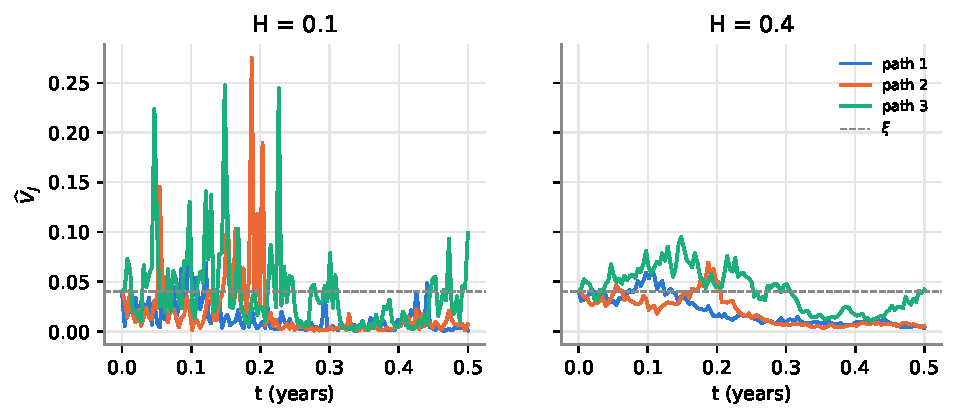
\includegraphics[width=0.85\textwidth]{../figures/p1c_variance_paths.pdf}
\caption{$\Vh_j$, $n=128$, $\xi=0.04$, $\eta=1.5$; same Gaussian inputs in both panels.}\label{fig:vpaths}
\end{figure}

\subsection*{(d)}
With $\eta=0$, (11) gives $\Vh_j=\xi$ for every $j$, whatever $\Yh_j$ and $q_j$ are. Summing (12),
\[
\log\Sh_n=\log S_0-\tfrac12\xi T+\sqrt\xi\sum_{j=1}^n\big(\rho\,\Delta W_j+\sqrt{1-\rho^2}\,\Delta B_j\big).
\]
The sum is Gaussian with mean $0$ and variance $n\Delta(\rho^2+1-\rho^2)=T$, so
$\log \Sh_n\sim N(\log S_0-\tfrac12\xi T,\ \xi T)$ exactly, for every $n$: this is the Black--Scholes
terminal law with zero rates and volatility $\sqrt\xi$. Hence $\E[(K-\Sh_n)^+]=\mathrm{BS}_{\rm put}(S_0,K,\xi T)$.
Table~\ref{tab:p1d}: $100{,}000$ paths per $n$, independent streams for each $n$; all $|z|\le2.02$.
\begin{table}[H]\centering\small
\input{\R/p1d_eta0_bs.tex}
\caption{$\eta=0$: simulated put prices vs (6) with $a=\xi T$; $z=(\text{MC}-\text{BS})/\text{SE}$.
The three strikes at a given $n$ share paths.}\label{tab:p1d}
\end{table}
\textbf{A bug these checks detect:} driving $\Delta B$ with the same normals as $\Delta W$ (a
dependence bug). The return variance becomes $(\rho+\sqrt{1-\rho^2})^2T\neq T$ and the prices move
far from (6). Wrong increment scaling or a missing $-\frac12\Vh_j\Delta$ term is caught the same way.

\textbf{A bug they do not detect:} anything in the variance driver, e.g.\ an off-by-one in the
convolution index ($\Delta W_{j-k+2}$ instead of $\Delta W_{j-k+1}$) or look-ahead (using
$\Vh_{j+1}$ in (12)). At $\eta=0$ the variance path is constant, so these errors have no effect.

%=====================================================================
\section*{Problem 2. A Black--Scholes control variate}

\subsection*{(a)}
By the argument of 1(d), $\log\widetilde S_T\sim N(\log S_0-\tfrac12\xi T,\xi T)$, so
\[
c_K=\E[C_K]=\mathrm{BS}_{\rm put}(S_0,K,\xi T).
\]
For fixed $\beta$: $\E[R]=\E[X]-\beta(\E[C]-c_K)=p_{K,n}$. Its variance is
$\Var(R)=\Var X-2\beta\Cov(X,C)+\beta^2\Var C$, a quadratic in $\beta$ minimised at
\[
\beta^*=\frac{\Cov(X,C)}{\Var C},\qquad \Var(R^*)=\Var X\,\big(1-\Corr(X,C)^2\big).
\]
If $\widetilde S_T$ were simulated independently, $\Cov(X,C)=0$, so $\beta^*=0$ and the control gives
no reduction; any $\beta\ne0$ adds $\beta^2\Var C$. The control only helps through its
correlation with $X$, which comes from sharing the increments $\Delta W_j,\Delta B_j$.

\subsection*{(b)}
$\hat\beta_K=\widehat{\Cov}(X,C)/\widehat{\Var}(C)$ is computed from an independent pilot and frozen.
Conditional on the pilot, $\hat\beta_K$ is a constant and the production $R_i$ are i.i.d.\ with
$\E[R_i\mid\text{pilot}]=p_{K,n}-\hat\beta_K(\E[C]-c_K)=p_{K,n}$. So the estimator is unbiased
conditional on the pilot, and (18) is the correct SE, because the $R_i$ are i.i.d.\ given the pilot.

If $\hat\beta$ is fitted on the production sample, it depends on the same $C_i$, and
$\E[\hat\beta(\bar C-c_K)]\neq0$ in general: the estimator has an $O(1/m)$ bias. The $R_i$ are also
no longer independent (all share $\hat\beta$), so (18) is justified only asymptotically.

\textbf{Zero pilot control variance.} If the pilot sample variance of $C$ is zero (e.g.\ all pilot
controls equal zero), the code sets $\hat\beta=0$, so the estimator reduces to plain Monte Carlo
(\texttt{\_coef} in \texttt{src/estimators.py}). This did not occur in any run.

\subsection*{(c)}
Implemented in \texttt{control\_variate()}: pilot of $10{,}000$ paths, then production
$R_i=X_i-\hat\beta(C_i-c_K)$ with SE and the 95\% interval from (18), using production observations only.

\textbf{Pathwise identity at $\eta=0$.} Then $\Vh_j\equiv\xi$, and (12) and (14) give the same
$\log\Sh_n=\log\widetilde S_T$, so $X=C$ on every path and, with $\beta=1$, $R=c_K$.
Table~\ref{tab:p2c} (10{,}000 paths): $\max_i|R_i-c_K|\le10^{-13}$ (roundoff; the two logs are
accumulated in different orders, $\max|\Sh_n/\widetilde S_T-1|=1.1\times10^{-15}$).
\begin{table}[H]\centering\small
\input{\R/p2c_identity.tex}
\caption{$\eta=0$, $\beta=1$: adjusted payoffs are constant up to roundoff.}\label{tab:p2c}
\end{table}

\textbf{Why an estimated coefficient need not reduce variance.} From (a),
$\Var(R(\beta))-\Var(X)=\Var(C)\big[(\beta-\beta^*)^2-\beta^{*2}\big]$, so a fixed $\beta$ reduces
variance only if $|\beta-\beta^*|<|\beta^*|$. The pilot $\hat\beta$ is random and can fall outside
this range, especially with a small pilot or weak correlation. Even when it is inside, the
reduction is a statement about population variances: in a given finite production sample the
sample variance of $R$ can still exceed that of $X$ by chance.

%=====================================================================
\section*{Problem 3. Antithetic sampling}

\subsection*{(a)}
$Z=(G,U,D)$ is a vector of i.i.d.\ $N(0,1)$ entries, and the standard normal law is symmetric,
so $-Z\overset{d}{=}Z$. $X^\pm$ are the same measurable function of $\pm Z$, so
$X^-\overset{d}{=}X^+$, the correct law. $\Yh_j$ is linear in $(G,U)$, so negation gives $-\Yh_j$, and
\[
\Vh_j^+=\xi\exp\!\big(\eta\Yh_j-\tfrac{\eta^2}{2}q_j\big),\qquad
\Vh_j^-=\xi\exp\!\big(-\eta\Yh_j-\tfrac{\eta^2}{2}q_j\big).
\]
Negating only the stock-return increments while keeping $\Vh^+$ drives the second stock with
$-\Delta W$ but a variance path built from $+\Delta W$. The pair (stock driver, variance driver) then
has correlation $-\rho$ instead of $\rho$, so the second path does not have the model's law (for
$\rho\neq0$). It is not the full reflection $Z\mapsto-Z$, under which the variance path changes too.

\subsection*{(b)}
Let $\sigma^2=\Var X^+=\Var X^-$ and $r=\Corr(X^+,X^-)$. For $M$ i.i.d.\ pair averages,
\[
\Var(\bar A_M)=\frac{\Var(A)}{M}=\frac{\sigma^2+\sigma^2+2r\sigma^2}{4M}=\frac{\sigma^2(1+r)}{2M},
\qquad \Var(\bar X_{2M})=\frac{\sigma^2}{2M},
\]
\[
\frac{\Var(\bar A_M)}{\Var(\bar X_{2M})}=1+\Corr(X^+,X^-).
\]
Antithetic sampling reduces variance iff $\Corr(X^+,X^-)<0$. This is \emph{not} guaranteed here. The
guarantee holds when the payoff is a monotone function of each input, and $Z\mapsto X$ is not. Raising
$G_j$ moves the stock through the $\rho\,\Delta W$ term (down, since $\rho<0$) and also raises
later variances through $\Yh$ (exponentially), which changes both the drift $-\frac12\Vh\Delta$ and the
size of subsequent returns. The put payoff also has a kink. With the even (variance-driven) part of
$X$ dominant, e.g.\ large $\eta$ and a far out-of-the-money strike, $r$ can be close to zero or positive.

\subsection*{(c)}
Implemented in \texttt{antithetic()}: each batch draws one $(G,U,D)$ per pair and simulates $Z$ and
$-Z$. The statistic is the pair average $A_i$, $i=1,\dots,M$; $\widehat{SE}=\sqrt{s_A^2/M}$ and the 95\%
interval follow (18) with $m=M$.

Treating the $2M$ payoffs as independent uses $s_X^2/(2M)$, which estimates $\sigma^2/(2M)$ and omits
the within-pair covariance term $2r\sigma^2/(4M)$. The true variance is $\sigma^2(1+r)/(2M)$. The naive
SE is therefore off by the factor $\sqrt{1+r}$: too large when $r<0$, too small when $r>0$. Only the
pairs are independent sampling units.

%=====================================================================
\section*{Problem 4. Combining the two methods}

\subsection*{(a)}
$\Var(R_{\rm pair})=\Var A-2\gamma\Cov(A,C_A)+\gamma^2\Var C_A$, minimised at
\[
\gamma^*=\frac{\Cov(A,C_A)}{\Var(C_A)},\qquad \Var(R^*_{\rm pair})=\Var A\,\big(1-\Corr(A,C_A)^2\big).
\]
Write each payoff as even plus odd parts in $Z$: $X=X_e+X_o$ with
$X_e(Z)=\frac12(X(Z)+X(-Z))$, $X_o(Z)=\frac12(X(Z)-X(-Z))$, and likewise $C$. Since $Z\overset d=-Z$, even
and odd functions are uncorrelated, so
\[
\beta^*=\frac{\Cov(X_e,C_e)+\Cov(X_o,C_o)}{\Var C_e+\Var C_o},\qquad
\gamma^*=\frac{\Cov(X_e,C_e)}{\Var C_e}\qquad(A=X_e,\ C_A=C_e).
\]
$\beta^*$ is a variance-weighted mix of the even and odd regression slopes. $\gamma^*$ is the even slope
alone, because pairing has already removed the odd parts. They coincide only if the two slopes are equal.

\subsection*{(b)}
Implemented in \texttt{combined()}: pilot of $5{,}000$ independent pairs gives $\hat\gamma$, frozen for
$M=50{,}000$ production pairs; $\widehat{SE}=\sqrt{s^2_{R_{\rm pair}}/M}$, where $s^2_{R_{\rm pair}}$ is the
sample variance of the $M$ production values $R_{{\rm pair},i}$.

\textbf{Unbiasedness given the pilot.} Each $C(\pm Z)$ has the law of $C$, so $\E[C_A]=c_K$. Given
the pilot, $\hat\gamma$ is constant and $\E[R_{\rm pair}\mid\text{pilot}]=\E[A]-\hat\gamma(\E[C_A]-c_K)=p_{K,n}$.
Numerically, the production mean of $C_A$ differs from $c_K$ by $\CtrlZBOTHa$, $\CtrlZBOTHb$, $\CtrlZBOTHc$ SE at
$K=90,100,110$, consistent with $\E[C_A]=c_K$. Every combined estimate lies inside the
plain-MC 95\% interval (Table~\ref{tab:prices}).

%=====================================================================
\section*{Problem 5. Numerical investigation}

\subsection*{(a) Baseline comparison}
Parameters (5), $n=128$; $100{,}000$ production path evaluations per method (paired methods: $50{,}000$
pairs); pilots of $10{,}000$ paths (CV) and $5{,}000$ pairs (AV+CV). Each method uses its own
independent streams, and all three strikes are evaluated on the same paths within a method.
\begin{table}[H]\centering\small
\input{\R/p5a_prices.tex}
\caption{Estimates, SE and 95\% intervals from (18); $m$ = production observations (paths or pairs).}\label{tab:prices}
\end{table}
\begin{table}[H]\centering\small
\input{\R/p5a_timing.tex}
\caption{Computation time per method, shared by all three strikes (counted once). Pilot and production
times are medians of 5 repeated runs with identical seeds (identical estimates); the last column is the
range of the 5 totals. Timing follows the protocol: it includes RNG, simulation, control evaluation,
coefficient estimation and production statistics, and excludes plotting, file output and a one-time warm-up.}\label{tab:time}
\end{table}
\begin{table}[H]\centering\small
\input{\R/p5a_efficiency.tex}
\caption{Fitted coefficients ($\hat\beta$ for CV, $\hat\gamma$ for AV+CV, from the pilot), production-sample
correlations, VRF and Gain from (19) using the total times of Table~\ref{tab:time}.
VRF$_{\rm pred}$ is the large-sample value implied by the correlations: $1/(1-\rho_{X,C}^2)$,
$1/(1+\rho_{X^+,X^-})$, $1/[(1+\rho_{X^+,X^-})(1-\rho_{A,C_A}^2)]$.}\label{tab:eff}
\end{table}

\subsection*{(b) Explanation}
\begin{figure}[H]\centering
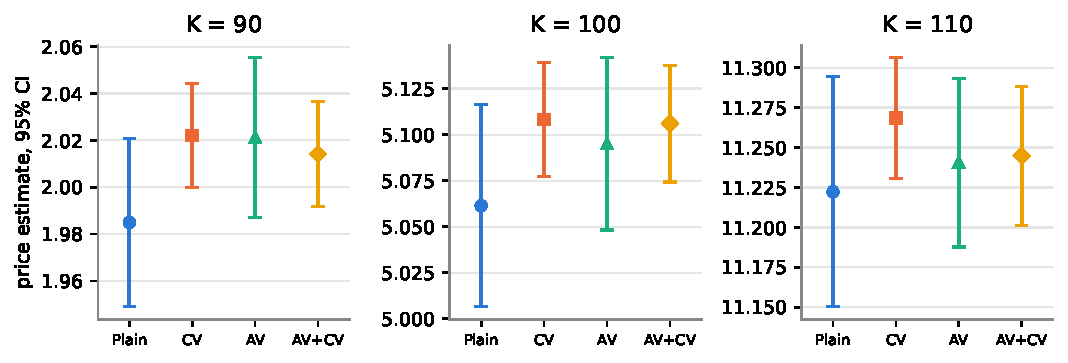
\includegraphics[width=0.95\textwidth]{../figures/p5b_ci.pdf}
\caption{95\% confidence intervals of the four estimators, baseline parameters (5), $n=128$.}\label{fig:ci}
\end{figure}
All intervals overlap at every strike (Figure~\ref{fig:ci}). Plain MC sits below the others at all
three strikes; its three estimates share paths, so their errors are positively correlated.

\textbf{Control variate.} $\rho_{X,C}=\RhoXCCVa,\RhoXCCVb,\RhoXCCVc$ at $K=90,100,110$, giving observed VRF $\VRFCVa,\VRFCVb,\VRFCVc$,
close to $1/(1-\rho^2)$. The control uses the same Brownian increments with variance frozen at $\xi$,
so it tracks the stock-noise part of $X$. The correlation rises with $K$: the in-the-money put is
closer to linear in $S_T$, while the out-of-the-money put depends more on the tails, where the
rough variance path matters most.

\textbf{Antithetic.} $\rho_{X^+,X^-}=\RhoPairAVa,\RhoPairAVb,\RhoPairAVc$, giving VRF $\VRFAVa,\VRFAVb,\VRFAVc\approx1/(1+\rho)$.
Reflection cancels the odd part of $X$ in $Z$; the payoff is closer to odd (linear) in $Z$ in the
money, so the gain grows with $K$.

\textbf{Combination.} VRF $\VRFBOTHa,\VRFBOTHb,\VRFBOTHc$: better than AV alone, but slightly \emph{below} CV alone at
every strike. Pairing removes the odd part of $X$, and that is mostly what the control also explains
(the control is driven by the same increments). The control is left to explain the even part,
which it does worse: $\rho_{A,C_A}=\RhoACABOTHa,\RhoACABOTHb,\RhoACABOTHc<\rho_{X,C}$. Hence
$(1+\rho_{X^+,X^-})(1-\rho_{A,C_A}^2)$ is not smaller than $1-\rho_{X,C}^2$; the two reductions overlap
rather than multiply. The fitted $\hat\gamma\neq\hat\beta$ (e.g.\ $\CoefBOTHc$ vs $\CoefCVc$ at $K=110$), as
4(a) predicts.

\textbf{Efficiency and ranking.} By VRF: CV $>$ AV+CV $>$ AV at every strike. By Gain the order
changes, because cost per path evaluation differs. AV draws one set of normals for two paths and
needs no control, so it is cheapest (\TimeAV\,s vs \TimePL\,s for plain). CV evaluates the control and runs
a pilot (\TimeCV\,s). AV+CV saves on random numbers and pays for the control (\TimeBOTH\,s). Hence Gain is
\{CV \GainCVa, AV \GainAVa, AV+CV \GainBOTHa\} at $K=90$, \{\GainCVb, \GainAVb, \GainBOTHb\} at $K=100$, and
\{\GainCVc, \GainAVc, \GainBOTHc\} at $K=110$. \textbf{The most efficient method by (19) is AV+CV at $K=90$ and
$K=100$.} At $K=110$ the three Gains differ by at most \GainSpreadc\%, comparable to the run-to-run timing
variability (Table~\ref{tab:time}), so no method is clearly most efficient there. The disagreement between VRF and Gain rankings comes entirely from
random-number generation cost: in this NumPy implementation it is a large share of the work, and
antithetic sampling halves it. A different implementation or hardware would change the time ratios
but not the VRFs.

\subsection*{(c) Parameter sensitivity ($K=100$, $n=128$)}
$100{,}000$ production path evaluations per method, pilots as in (a), one parameter changed at a time.
\begin{table}[H]\centering\small
\input{\R/p5c_sensitivity.tex}
\caption{$K=100$; coef.\ is $\hat\beta$ (CV) or $\hat\gamma$ (AV+CV). Baseline values at $K=100$: VRF CV 3.16,
AV \VRFAVb, AV+CV \VRFBOTHb; Gain \GainCVb, \GainAVb, \GainBOTHb.}\label{tab:sens}
\end{table}
\textbf{$\eta=0.5$.} Weaker variance fluctuations make $\Sh_n$ close to the Black--Scholes control:
$\rho_{X,C}$ rises from $\RhoXCCVb$ to $\SERhoXCCV$ and the CV VRF from $\VRFCVb$ to $\SEVRFCV$. The pair correlation also
becomes more negative ($\RhoPairAVb\to\SERhoPairAV$), since the payoff is closer to odd in $Z$. After pairing, the
control still explains the even part well ($\rho_{A,C_A}=\SERhoACABOTH$), so the combination now beats each
method separately (VRF \SEVRFBOTH, Gain \SEGainBOTH, the most efficient).

\textbf{$H=0.4$.} Smoother variance paths give a milder improvement: $\rho_{X,C}=\SHRhoXCCV$ (CV VRF \SHVRFCV),
$\rho_{X^+,X^-}=\SHRhoPairAV$ (AV VRF \SHVRFAV) and $\rho_{A,C_A}=\SHRhoACABOTH$. The combination again improves on both
(VRF \SHVRFBOTH, Gain \SHGainBOTH, the most efficient). In both cases the relative timing of methods is unchanged
from the baseline (Gain $\approx$ VRF $\times$ cost ratio), so the efficiency changes come from the
correlations.

\subsection*{(d) Reproducibility and implementation}
\begin{itemize}\itemsep0pt
\item \textbf{Software/hardware:} Python 3.11.15, NumPy 2.4.4, SciPy 1.17.1 (Matplotlib for figures);
Linux x86\_64, Intel Xeon @ 2.80\,GHz, 2 logical CPUs; float64 throughout
(\texttt{results/environment.json}).
\item \textbf{Seeds:} every stream is \texttt{PCG64(SeedSequence(9821, spawn\_key=key))}. Keys: 1(c)
moments $(1,3)$, 1(c) plot $(1,4)$, 1(d) $(1,5,i)$ for the $i$-th $n$, 2(c) $(1,6)$; Problem 5(a)
$(5,\text{method},\text{stage})$ with method $\in\{0,1,2,3\}$ = Plain, CV, AV, AV+CV and stage $0$ =
pilot, $1$ = production; 5(c) $(60,\cdot,\cdot)$ for $\eta=0.5$ and $(61,\cdot,\cdot)$ for $H=0.4$;
Bonus $(7,0,1)$. Within a batch the normals are drawn as $G$, then $U$, then $D$, each of shape
(batch, $n$).
\item \textbf{Batching:} $10{,}000$ path evaluations per batch ($5{,}000$ pairs for paired methods).
Means and co-moment matrices are combined across batches with the pairwise (Chan et al.) update;
no path arrays are stored.
\item \textbf{Pilot vs production:} each method has distinct spawn keys for pilot and production,
so the two streams are independent, and the coefficient is computed and frozen before any
production draw.
\item \textbf{Pairs as units:} one row of $(G,U,D)$ is drawn per pair; the two members are $Z$ and $-Z$
of that row. Statistics are accumulated on the pair average (or adjusted pair average), so each pair
contributes one observation, and $m=M$ in (18).
\end{itemize}

%=====================================================================
\section*{Bonus. Conditional Monte Carlo}

\subsection*{(a)}
Let $\mathcal G=\sigma(G_1,\dots,G_n,U_1,\dots,U_n)$. Then $\Vh_0,\dots,\Vh_{n-1}$, $I_n$ and $J_n$ are
$\mathcal G$-measurable, and summing (12) gives
\[
\log\Sh_n=\log S_0-\tfrac12 I_n+\rho J_n+\sqrt{1-\rho^2}\sum_{j=0}^{n-1}\sqrt{\Vh_j}\,\Delta B_{j+1}.
\]
The $\Delta B$ are independent of $\mathcal G$, so given $\mathcal G$ the last sum is $N(0,I_n)$, and
\[
\log\Sh_n\mid\mathcal G\sim N\big(\log S_0+\rho J_n-\tfrac12 I_n,\ (1-\rho^2)I_n\big).
\]
With $s^*=S_0\exp(\rho J_n-\tfrac{\rho^2}{2}I_n)$ and $a=(1-\rho^2)I_n$, the mean is
$\log s^*-\frac12 a$. This is the Black--Scholes law with spot $s^*$ and total variance $a$, so
$Q_K=\E[(K-\Sh_n)^+\mid\mathcal G]=\mathrm{BS}_{\rm put}(s^*,K,a)$, which is (21).
Using $S_0$ as the spot ignores the $\mathcal G$-measurable shift $\rho J_n-\frac{\rho^2}{2}I_n$, i.e.\
the part of the return driven by the same $W$ as the variance. It is correct only if $\rho=0$.

\subsection*{(b)}
By the law of total variance,
$\Var X_K^{(n)}=\E[\Var(X_K^{(n)}\mid\mathcal G)]+\Var(Q_K)\ge\Var(Q_K)$, with the gap equal to the
average conditional variance from the $D$ noise. Reflecting only $D$ (keeping $G,U$) gives the pair
average $\frac12\big(X(G,U,D)+X(G,U,-D)\big)$. Its conditional mean is also $Q_K$, and it removes the part
of the $D$-noise that is odd in $D$. Exact conditional averaging integrates over $D$ completely and
removes all of it; $D$-reflection is a two-point approximation of that integral.

\subsection*{(c)}
$100{,}000$ independent $(G,U)$ samples, baseline (5), $K=100$, $n=128$; time is the median of 5 runs.
\begin{table}[H]\centering\small
\input{\R/bonus_conditional.tex}
\caption{$K=100$: conditional estimator vs the four methods of 5(a); VRF and Gain relative to plain MC.}
\end{table}
The conditional estimator has VRF \VRFCOND\ and Gain \GainCOND, against Gains \GainCVb\ (CV), \GainAVb\ (AV)
and \GainBOTHb\ (AV+CV): better than AV, below AV+CV. Its VRF is limited because it removes only the independent stock noise
(weight $1-\rho^2=0.51$); the variance-path and $\rho J_n$ noise remain.

\textbf{Cost per sample.} One sample needs no $D$ draws (two thirds of the normals) and no stock
recursion (12). It needs the variance path, two sums $I_n,J_n$, and one Black--Scholes formula per
strike, so it is cheaper than a full stock path (\TimeCOND\,s vs \TimePL\,s per $100{,}000$).

\end{document}
